%%
% このファイルは、筑波大学情報学群情報メディア創成学類の
% 卒業研究論文本体のサンプルです。
% このファイルを書き換えて、この例と同じような書式の論文本体を
% LaTeXを使って作成することができます。
%
% PC環境や、LaTeX環境の設定によっては漢字コードや改行コードを
% 変更する必要があります。
%%
\documentclass[a4paper,11pt]{jreport}

%%【PostScript, JPEG, PNG等の画像の貼り込み】
%% 利用するパッケージを選んでコメントアウトしてください。
%\usepackage{graphicx} % for 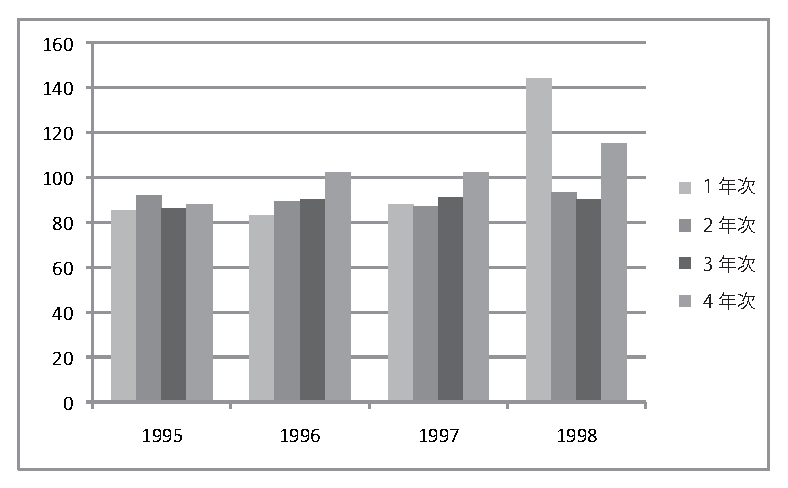
\includegraphics[width=3cm]{sample.eps}
\usepackage{epsfig} % for 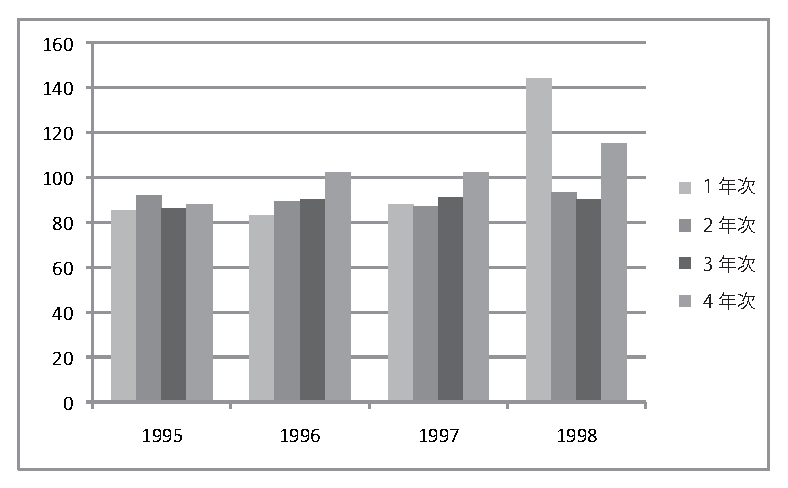
\psfig{file=sample.eps,width=3cm}
%\usepackage{epsf} % for \epsfile{file=sample.eps,scale=0.6}
%\usepackage{epsbox} % for \epsfile{file=sample.eps,scale=0.6}

\usepackage{times} % use Times Font instead of Computer Modern

\setcounter{tocdepth}{3}
\setcounter{page}{-1}

\setlength{\oddsidemargin}{0.1in}
\setlength{\evensidemargin}{0.1in}
\setlength{\topmargin}{0in}
\setlength{\textwidth}{6in}
%\setlength{\textheight}{10.1in}
\setlength{\parskip}{0em}
\setlength{\topsep}{0em}

%\newcommand{\zu}[1]{{\gt \bf 図\ref{#1}}}

%% タイトル生成用パッケージ(重要)
\usepackage{mast-utf}

%% タイトル
%% 【注意】タイトルの最後に\\ を入れるとエラーになります
\title{卒業論文の書き方}
%% 著者
\author{筑波 太郎}
%% 指導教員
\advisor{筑波 大二郎}

%% 年月 (提出年月)
%% 年月は必要に応じて書き替えてください。
\majorfield{ } \yearandmonth{2018年 1月}



\begin{document}
\maketitle
\thispagestyle{empty}
\newpage

\thispagestyle{empty}
\vspace*{20pt plus 1fil}
\parindent=1zw
\noindent
%%
%% 論文の概要(Abstract)
%%
\begin{center}
{\bf 概要}
\vspace{5mm}
\end{center}
この文書は、筑波大学情報学群情報メディア創成学類の卒業研究論文本体のサンプル
である。このファイルを書き換えて、この例と同じような書式の論文本体を
\LaTeX を使って作成することができる。

このサンプルは、学生諸君が面倒な位置決めをして表紙を作成する手間を軽減す
るために提供している。もちろん、このサンプルで示す表紙は例であり、要項に
準拠していれば、このファイルに頼らずに自分で表紙の位置決めを行ってもよい。

%%%%%
\par
\vspace{0pt plus 1fil}
\newpage

\pagenumbering{roman} % I, II, III, IV
\tableofcontents
\listoffigures
%\listoftables

\pagebreak \setcounter{page}{1}
\pagenumbering{arabic} % 1,2,3


\chapter{はじめに}

研究の内容や分野によっては書き方が異なる場合もあるので、詳しいことは指導教員に聞くと
よい。この文書は主にタイトルの作成方法と、論文の体裁を示すのみであり、どうやっ
たらよい論文になるかの示唆は含まれていない。

\chapter{形式}

ここでは、論文の表紙および本体の記述方法について述べる。

\section{表紙}

表紙は、{\tt $\backslash$maketitle} によって作成するため、以下の項目に相
当する文字列をそれぞれ記述する。

\begin{description} \parskip=1pt
\item{題目: }
題目は{\tt $\backslash$title} に記述する。行替えを行う場合は$\backslash$
	   $\backslash$ を入力する。ただし、題目の最後に$\backslash$
	   $\backslash$ を入力するとコンパイルが通らなくなるので注意する。
	   なお、4行以上の題目の場合、表紙ページがあふれるためスタイルファ
	   イル``mast-jp-sjis.sty''を変更する必要がある。
\item{著者名: }
著者名は{\tt $\backslash$author} に記述する。
\item{指導教員名: }
指導教教員は{\tt $\backslash$advisor} に記述する。
\item{年月: }
年月は{\tt $\backslash$yearandmonth} に記述する。年月は提出時のものを記述すること。
\end{description}

\section{本体}

本体は1段組で記述する。

図表には番号と説明(caption)を付け、文章中で参照する。表
\ref{table:fundamental_data_type}と図\ref{figure:sample}はそれぞれ表と図
の例である。表の説明は上に、図の説明は下に書くことが多い。図の挿入に用い
るパッケージについては使用環境に合わせて自由に選択してほしい。

\begin{table}[hbt]
\caption{表の例}
\label{table:fundamental_data_type}
\begin{center}
\begin{tabular}{| c | r | r | r | r |}
\hline
年 度 & 1年次 & 2年次 & 3年次 & 4年次 \\
\hline
1995 & 85 & 92 & 86 & 88 \\
1996 & 83 & 89 & 90 & 102 \\
1997 & 88 & 87 & 91 & 112 \\
1998 & 144 & 93 & 90 & 115 \\
\hline
\end{tabular}
\end{center}
\end{table}
\medskip

\begin{figure}[htbp]
\begin{center}
%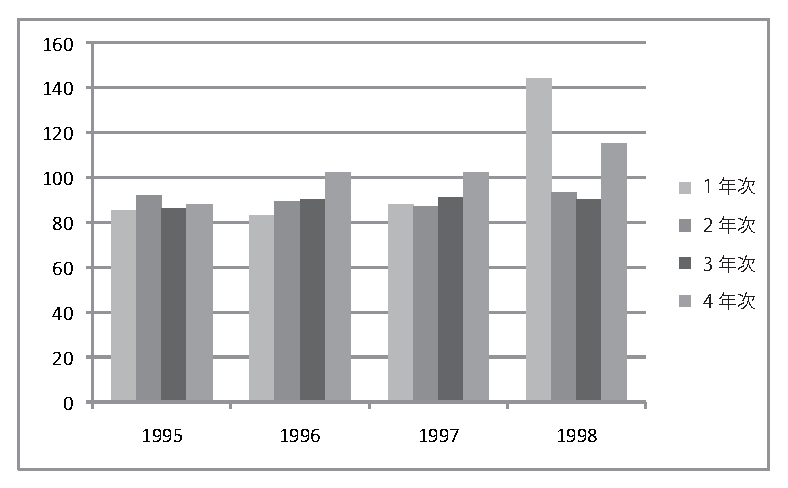
\includegraphics[width=3cm]{sample.eps}
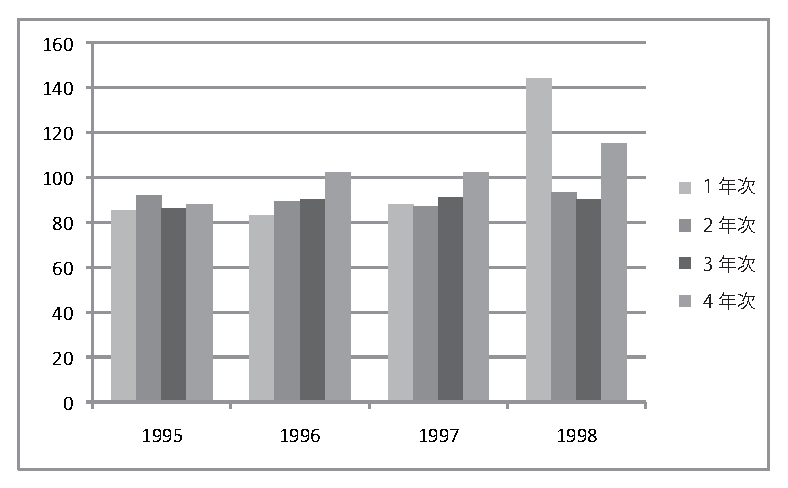
\psfig{file=sample.eps,scale=0.6}
%\epsfile{file=sample.eps,scale=0.6}
\end{center}
\caption{図の例}
\label{figure:sample}
\end{figure}

詳しくは参考書\cite{okumura2010,yoshinaga2009}などを参照のこと。
また、奥村晴彦氏の「\TeX Wiki」
http://oku.edu.mie-u.ac.jp/\textasciitilde{}okumura/texwiki/
は、日本語の\TeX に関する情報が充実している。
また、具体的な論文としての文献参照例として
(本の例)\cite{ware2004}、
(雑誌論文の例)\cite{meyer2009}、
(予稿集の例)\cite{hill2010}
を挙げておく。

\chapter*{謝辞}
\addcontentsline{toc}{chapter}{\numberline{}謝辞}

\newpage

\addcontentsline{toc}{chapter}{\numberline{}参考文献}
\renewcommand{\bibname}{参考文献}

%% 参考文献に jbibtex を使う場合
%\bibliographystyle{junsrt}
%\bibliography{samplebib}
%% [compile] jbibtex sample; platex sample; platex sample;

%% 参考文献を直接ファイルに含めて書く場合
\begin{thebibliography}{1}
\bibitem{okumura2010}
奥村晴彦, LaTeX2e美文書作成入門 改訂第5版, 技術評論社, 2010年.

\bibitem{yoshinaga2009}
吉永徹美, LaTeX2ε辞典, 翔泳社, 2009年.

\bibitem{ware2004}
Colin Ware, Information Visualization --- Perception for Design, Second Edition, Morgan Kaufmann Publishers, 486‾p., 2004.

\bibitem{meyer2009}
Miriah Meyer and Tamara Munzner, MizBee: A Multiscale Synteny Browser, {\em IEEE Transactions on Visualization and Computer Graphics}, Vol.‾15, No.‾6, pp.‾897--904, 2009.

\bibitem{hill2010}
Emerson Murphy-Hill and Andrew P. Plack, An Interactive Ambient Visualization for Code Smells, {\em in Proceedings of the 2010 International Symposium on Software Visualization (SOFTVIS’10)}, pp.‾5--14, 2010.

\end{thebibliography}

\end{document}
